\documentclass{standalone}
\usepackage{tikz}
\usetikzlibrary{arrows.meta}

\begin{document}

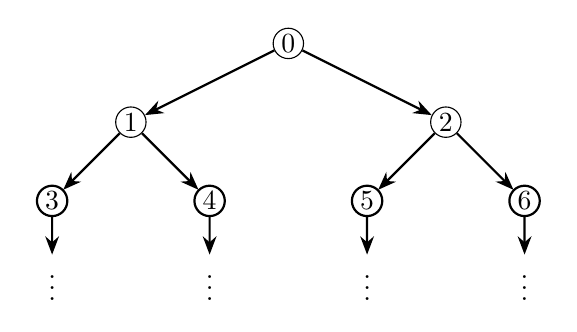
\begin{tikzpicture}[
    level 1/.style={sibling distance=40mm},
    level 2/.style={sibling distance=20mm},
    level 3/.style={sibling distance=10mm},
    every node/.style={circle, draw, inner sep=1pt},
    edge from parent/.style={draw, thick, -{Stealth[]}},
    level distance=10mm
    ]

    \node {0}
        child {node {1}
            child {node {3}
                child {node [draw=none] {$\vdots$}}
            }
            child {node {4}
                child {node [draw=none] {$\vdots$}}
            }
        }
        child {node {2}
            child {node {5}
                child {node [draw=none] {$\vdots$}}
            }
            child {node {6}
                child {node [draw=none] {$\vdots$}}
            }
        };
\end{tikzpicture}

\end{document}